%% This is file `elsarticle-template-1-num.tex',
%%
%% Copyright 2009 Elsevier Ltd
%%
%% This file is part of the 'Elsarticle Bundle'.
%% ---------------------------------------------
%%
%% It may be distributed under the conditions of the LaTeX Project Public
%% License, either version 1.2 of this license or (at your option) any
%% later version.  The latest version of this license is in
%%    http://www.latex-project.org/lppl.txt
%% and version 1.2 or later is part of all distributions of LaTeX
%% version 1999/12/01 or later.
%%
%% The list of all files belonging to the 'Elsarticle Bundle' is
%% given in the file `manifest.txt'.
%%
%% Template article for Elsevier's document class `elsarticle'
%% with numbered style bibliographic references
%%
%% $Id: elsarticle-template-1-num.tex 149 2009-10-08 05:01:15Z rishi $
%% $URL: http://lenova.river-valley.com/svn/elsbst/trunk/elsarticle-template-1-num.tex $
%%
\documentclass[preprint,12pt]{elsarticle}

%% Use the option review to obtain double line spacing
%% \documentclass[preprint,review,12pt]{elsarticle}

%% Use the options 1p,twocolumn; 3p; 3p,twocolumn; 5p; or 5p,twocolumn
%% for a journal layout:
%% \documentclass[final,1p,times]{elsarticle}
%% \documentclass[final,1p,times,twocolumn]{elsarticle}
%% \documentclass[final,3p,times]{elsarticle}
%% \documentclass[final,3p,times,twocolumn]{elsarticle}
%% \documentclass[final,5p,times]{elsarticle}
%% \documentclass[final,5p,times,twocolumn]{elsarticle}

%% if you use PostScript figures in your article
%% use the graphics package for simple commands
%% \usepackage{graphics}
%% or use the graphicx package for more complicated commands
\usepackage{graphicx}
%% or use the epsfig package if you prefer to use the old commands
%% \usepackage{epsfig}

\usepackage{oubraces}
\usepackage{epstopdf}

\usepackage{amssymb,amsmath}
%\usepackage{amsthm}
\usepackage{url}
\usepackage{psfrag}
\usepackage{color}
\usepackage{hyperref}
\usepackage{breakurl}
%\usepackage[dvips]{graphics,graphicx}
%\usepackage[dvips]{graphicx}
\usepackage{rotating}

\usepackage{verbatimbox}
\usepackage{epsfig}
\usepackage{chngpage}

%% The amssymb package provides various useful mathematical symbols
\usepackage{amssymb}
%% The amsthm package provides extended theorem environments
%% \usepackage{amsthm}

%% The lineno packages adds line numbers. Start line numbering with
%% \begin{linenumbers}, end it with \end{linenumbers}. Or switch it on
%% for the whole article with \linenumbers after \end{frontmatter}.
%% \usepackage{lineno}

%% natbib.sty is loaded by default. However, natbib options can be
%% provided with \biboptions{...} command. Following options are
%% valid:

%%   round  -  round parentheses are used (default)
%%   square -  square brackets are used   [option]
%%   curly  -  curly braces are used      {option}
%%   angle  -  angle brackets are used    <option>
%%   semicolon  -  multiple citations separated by semi-colon
%%   colon  - same as semicolon, an earlier confusion
%%   comma  -  separated by comma
%%   numbers-  selects numerical citations
%%   super  -  numerical citations as superscripts
%%   sort   -  sorts multiple citations according to order in ref. list
%%   sort&compress   -  like sort, but also compresses numerical citations
%%   compress - compresses without sorting
%%
%% \biboptions{comma,round}

% \biboptions{}


\journal{Nuclear Physics B}

\newcommand{\paral}{\; \vert \;}
\newcommand{\myvec}[1]{\overrightarrow{#1}}
\newcommand{\Defeq}{\stackrel{\mathrm{df}}{=}}
\newcommand{\Bnfeq}{::=}
\newcommand{\Co}[1]{\overline{#1}}

%
\newcommand{\Bsep}{\: \mid \: }
\newcommand{\Rule}[2]{\displaystyle{\frac{#1}{#2}}}
\newcommand{\SF}[1]{\mathsf{#1}}
\newcommand{\Act}{\mathsf{Act}}
\newcommand{\Vis}{\mathsf{Vis}}
\newcommand{\ActK}{\mathsf{ActK}}
\newcommand{\Proc}{\mathsf{Proc}}
\newcommand{\Procc}{\mathsf{ProcC}}
\newcommand{\Pred}{\mathsf{Pred}}
\newcommand{\Std}{\mathsf{Std}}
\newcommand{\rms}{\mathrm{S}}
\newcommand{\rmrec}{\mathrm{rec}}
\newcommand{\rmreck}{\mathrm{reck}}
\newcommand{\rmreckR}{\mathrm{reckR}}
\newcommand{\rma}{\mathrm{A}}
\newcommand{\rmp}{\mathrm{P}}
\newcommand{\rmf}{\mathrm{F}}
\newcommand{\rmr}{\mathrm{R}}
\newcommand{\rmfr}{\mathrm{FR}}
\newcommand{\equivS}{\equiv_{\mathrm{S}}}
\newcommand{\SigSA}{\Sigma_{\mathrm{SA}}}
\newcommand{\ltran}[1]{\stackrel{#1}{\longrightarrow}}
\newcommand{\tran}[1]{\stackrel{#1}{\rightarrow}}
\newcommand{\nottran}[1]{\stackrel{#1}{\not\rightarrow}}
\newcommand{\Rtran}[1]{\stackrel{#1}{\rightsquigarrow}}
\newcommand{\notRtran}[1]{\stackrel{#1}{\not\rightsquigarrow}}
\newcommand{\trans}[1]{\stackrel{#1}{\rightarrow}_{\mathrm{S}}}
\newcommand{\Par}{\mid}
\newcommand{\restrict}[1]{\!\setminus\!#1}

\newcommand{\mA}{\mathcal{A}}
\newcommand{\mSA}{\mathcal{SA}}
\newcommand{\mWA}{\mathcal{WA}}
\newcommand{\mAK}{\mathcal{AK}}
\newcommand{\umAK}{\underline{\mathcal{A}}\mathcal{K}}
\newcommand{\un}[1]{\underline {#1}}
\newcommand{\PI}{\mathcal{PI}}
\newcommand{\rom}[1]{\mbox{\rm{#1}}}

\newcommand{\Nil}{\mathbf{0}}
\newcommand{\New}[1]{\nu#1\: }
\newcommand{\Str}{\equiv}
\newcommand{\stdpred}{\mathsf{std}}
\newcommand{\std}[1]{\mathsf{std}(#1)}
%
\newcommand{\Bch}[2]{\mathsf{before}_{#1}(#2)}

\newcommand{\keys}[1]{\mathsf{keys}(#1)}
\newcommand{\kkey}[1]{\mathsf{k}(#1)}
\newcommand{\key}[1]{[#1]}
\newcommand{\Keys}{\mathcal{K}}
\newcommand{\freshpred}[1]{\mathsf{fsh}[#1]}
\newcommand{\fresh}[2]{\mathsf{fsh}[#1](#2)}

\newcommand{\ta}[1]{\mathsf{ta}(#1)}
\newcommand{\action}[1]{\mathsf{act}(#1)}

\newcommand{\intr}{\mbox{\ $\hat{}$\ }}
%\newcommand{\intr}{\mbox{\; $\widehat{}$\;}}
\newcommand{\sterm}{\mathsf{trm}}
\newcommand{\Sterm}[1]{\sterm(#1)}
\newcommand{\und}[1]{\underline{#1}}
\newcommand{\sqc}{\mathop{\cdot}}
\newcommand{\card}[1]{|#1|}
\newcommand{\bydef}{\stackrel{\emph{def}}{=}}
%
\newcommand{\Angle}[1]{\langle #1 \rangle}
\newcommand{\Tri}{\triangleright}
\newcommand{\Hole}{\bullet}
\newcommand{\rec}[1]{\mathrm{rec}\, #1}
\newcommand{\Rec}[1]{\rec #1 .}
\newcommand{\Rch}{\mathsf{Rch}}
\newcommand{\prune}{\pi}
\newcommand{\Prune}[1]{\prune(#1)}
\newcommand{\Root}[1]{\mathsf{rt}(#1)}

\newcommand{\Bis}{\sim}
\newcommand{\Biss}{\Bis_{\mathsf{S}}}
\newcommand{\Bisf}{\Bis_{\mathsf{F}}}
\newcommand{\Bisfr}{\Bis_{\mathsf{FR}}}
%\newcommand{\Bisu}{\Bis_{\Un}}
\newcommand{\Sim}{\mathcal{S}}
\newcommand{\Rem}{\backslash}
\newcommand{\sqeqt}{\sim}
% rules:
% static rule
\newcommand{\one}{\mbox{(I)}}
\newcommand{\onef}{\mbox{(1)}}
\newcommand{\oner}{\mbox{(1R)}}
% choice rule
\newcommand{\two}{\mbox{(II)}}
\newcommand{\twof}{\mbox{(2)}}
\newcommand{\twor}{\mbox{(2R)}}
% choice axiom
\newcommand{\thr}{\mbox{(III)}}
\newcommand{\thrf}{\mbox{(3)}}
\newcommand{\thrr}{\mbox{(3R)}}
\newcommand{\thrpf}{\mbox{(3\,$'$\!)}}
\newcommand{\thrpr}{\mbox{(3\,$'$\!R)}}
%
%
\newcommand{\Draft}[1]{}
\newcommand{\Comment}[1]{}
\newcommand{\Rev}[1]{{#1}^{-1}}

\newtheorem{theorem}{Theorem}
\newtheorem{definition}{Definition}
\newtheorem{remark}{Remark}
\newtheorem{example}{Example}
\newtheorem{proposition}{Proposition}

\begin{document}

\begin{frontmatter}

%% Title, authors and addresses

%% use the tnoteref command within \title for footnotes;
%% use the tnotetext command for the associated footnote;
%% use the fnref command within \author or \address for footnotes;
%% use the fntext command for the associated footnote;
%% use the corref command within \author for corresponding author footnotes;
%% use the cortext command for the associated footnote;
%% use the ead command for the email address,
%% and the form \ead[url] for the home page:
%%
%% \title{Title\tnoteref{label1}}
%% \tnotetext[label1]{}
%% \author{Name\corref{cor1}\fnref{label2}}
%% \ead{email address}
%% \ead[url]{home page}
%% \fntext[label2]{}
%% \cortext[cor1]{}
%% \address{Address\fnref{label3}}
%% \fntext[label3]{}

\title{CCB, a calculus for local reversibility}

%% use optional labels to link authors explicitly to addresses:
%% \author[label1,label2]{<author name>}
%% \address[label1]{<address>}
%% \address[label2]{<address>}

\author{Stefan Kuhn, Irek Ulidowski}

\address{Department of Informatics, University of Leicester, Leicester, LE1 7RH, United Kingdom}

\begin{abstract}
We introduce a process calculus with a new prefixing operator that allows us to model 
locally controlled reversibility. 
Actions can be undone spontaneously, as in other reversible process calculi, or as pairs of concerted 
actions, where performing a weak action forces undoing of another action. The new operator in its 
full generality allows us to model out-of-causal order computation, where effects are undone 
before their causes are undone, which goes beyond what typical reversible calculi can express. 
However, the core calculus, with a restricted form of the new operator, is well behaved as it 
satisfied causal consistency.
We demonstrate the usefulness of the calculus by modelling the hydration of formaldehyde in water 
into methanediol, an industrially important reaction, where the creation and breaking of some 
bonds are examples of locally controlled out-of-causal order computation.
\end{abstract}

\begin{keyword}
Reversible process calculi \sep local reversibility \sep modelling of chemical reactions
\end{keyword}

\end{frontmatter}

%%
%% Start line numbering here if you want
%%
% \linenumbers

%% main text
\section{Introduction}
There are many different computation tasks which involve undoing of previously 
performed steps or actions. Consider a computation where the action $a$ causes the action $b$,
written $a<b$, and where the action $c$ occurs independently of $a$ and $b$.
There are three  executions of this computation that preserve \emph{causality},
namely $abc$, $acb$ and $cab$. We note that $a$ always comes before $b$.
There are several conceptually different ways of undoing these actions
\cite{UPY2014}. {\em Backtracking}
is undoing in precisely the reverse order in which they happened. So, undo $b$ undo $c$ undo
$a$ is a backtrack of the execution $acb$.
{\em Reversing\/} is a more general form of undoing: here actions can be undone in any
order provided causality is preserved (meaning that causes cannot be undone before effects).
For example, undo $c$ undo $b$ undo $a$ is a reversal of $acb$ for the events $a,b$ 
and $c$ above.


In biochemistry, however, there are networks of reactions
where actions are undone seemingly \emph{out of causal order}.
The creation and breaking of molecular bonds between the proteins involved
in the ERK signalling pathway is a good example 
of this phenomenon ~\cite{PUY12}. Let us assume for simplicity that the creation of molecular 
bonds is represented by actions $a,b,c$ where, as above, $a<b$ and $c$ is independent 
of $a$ and $b$. In the ERK pathway, the molecular bonds are broken in the following 
order: undo $a$, undo $b$, undo $c$, which seems to undo the cause $a$ before the effect $b$. 
The first process calculus for the out-of-causal order
reversible computation was proposed in \cite{PUY12}, where the calculus CCSK 
\cite{PhiUli07} which is extended with an \emph{execution control mechanism} for 
managing the pattern and the direction of computation. The control mechanism is external
to the processes it controls, and it can have a global scope. Out-of-causal order computation
was also studied in \cite{PUY13a,PU13b}.
Other reversible process 
calculi were proposed in \cite{DK04,DK07,PU06,PhiUli07,LaneseMS10,LMSS11,LMS12,CKV13}.

We introduced informally a novel and purely local in character mechanism for undoing
of computation in a short paper \cite{KU2015}. Here, we build a process calculus 
around this mechanism and give it operational semantics.
We then discuss various properties that hold in the calculus. Most importantly, 
we show that out-of-causal order computation can be modelled in the calculus. Hence, in general,
the \emph{causal consistency} property \cite{DK04} does not hold. There are reachable states 
that can only be arrived at by a mixture of forward and reverse steps. However, we argue that 
causal consistency holds in a restricted version of our calculus, thus the full calculus is in effect
a ``conceptual'' extension of a causally consistent reversible process calculus. The benefits
of the calculus are shown by modelling hydration of formaldehyde 
in water. The molecules of formaldehyde and water are modelled as compositions 
of carbon, oxygen and hydrogen atoms. When composed in parallel, the molecules react 
and the reactions are represented by sequences of transitions of \emph{concerted actions}. 
We are able to represent different forms of reversibility, including out-of-causal-order 
reversibility, and computation can proceed in any directions without without external control.

The novel features of our calculus are introduced via an example of catalytic reaction.
Consider two molecules $A$ and $B$ that are only able to bond if assisted by the catalyst $C$. 
We assume
	$A  \bydef  (a;p).A'$, $B  \bydef  (b,p).B'$ and $C \bydef  (a,b).C'$.
We use a new prefix operator $(s;p).P$ where $s$ is a sequence of actions or executed
actions and $p$ is a \emph{weak} action. Initially the actions in $s,p$ take place,
and then we compute with $P$.  The three molecules can bond by performing synchronously the
matching actions according to the function $\gamma(a,a)=c$, $\gamma(b,b)=d$ and
$\gamma(p,p)=q$, producing thus new actions $c,d$ and $q$. A weak action $p$ can be left out
resulting in the prefix $(s;p).P$ (as in $B$ and $C$ above).
Actions in $s$ can take place in any order, and $p$ can happen if
all actions in $s$ have already taken place. Once $p$ takes place, one of the executed
actions in $s$ must be undone immediately: this is our new mechanism for
triggering reverse computation.  We shall model these two almost simultaneous
events as a transition of concerted actions. This is
a simple but realistic representation of the mechanism of covalent bonding, 
the most common type of chemical bonds between atoms, hence our calculus is
called a \emph{Calculus of Covalent Bonding}.

Returning to our example, we represent the system of molecules $A,B$ and $C$ as 
$((a;p).A' \paral (b,p).B' \paral (a,b).C') \setminus \{a,b,p\}$, 
where `$\paral$' is the parallel composition and `$\setminus$' the restriction as in
CCS and ACP \cite{Mil80,BW90}.
We note that $A$ and $B$ cannot interact initially since $\gamma(a,b)$ is not defined. 
But they can both 
interact with $C$:
\begin{flalign*}
&(a;p).A' \paral (b,p).B' \paral (a,b).C' \xrightarrow{c[1]} (a[1];p).A' \paral (b,p).B' 
	\paral (a[1],b).C' \xrightarrow{d[2]} \\
&(a[1];p).A' \paral (b[2],p).B' \paral (a[1],b[2]).C'
\end{flalign*}
where 1 and 2 are communication keys \cite{PhiUli07} indicating which pairs of actions created bonds. 
Molecules $A$ and $B$ can now do $p$ synchronously, producing action $q$. This causes immediately 
the breaking of the bond $c$, which means undoing of actions $a$ in $A$ and $C$, leaving
$A$ and $B$ bonded. We model such pairs of events by pairs of concerted actions:
\begin{flalign*}
	&(a[1];p).A' \paral (b[2],p).B' \paral (a[1],b[2]).C' \\
	&\xrightarrow{\{q[3],\underline{c}[1]\}} (a;p[3]).A' \paral (b[2],p[3]).B' \paral (a,b[2]).C'
\end{flalign*}
The bond 3 on weak actions $p$ is unstable and thus gets \emph{promoted} to a stable stronger 
bond on $a$ and $p$. Finally, the catalyst dissolves the bond with $B$:
\begin{flalign*}
&(a;p[3]).A' \paral (b[2],p[3]).B' \paral (a,b[2]).C' \Rightarrow (a[3];p).A' \paral (b[2],p[3]).B' 
	\paral (a,b[2]).C'\\
&\xrightarrow{\underline{d}[2]} (a[3];p).A' \paral (b,p[3]).B' \paral (a,b).C'
\end{flalign*}
We note that $A$ and $B$ are now bonded although the synchronisation function did not allow 
it to happen initially. The main consequence of this is that the bond between $a[3]$ and $p[3]$ is 
\emph{irreversible}, namely it cannot be undone.
Looking at the pattern of doing and undoing of bonds we obtain $c[1] d[2] 
q[3] \underline{c}[1] \underline{d}[2]$. Since creation of bonds $c$ and $d$ causes the bond $q$, 
we have here an example of out-of-causal order computation.

Biochemical reactions can also be modelled, for example, with the kappa calculus \cite{danos2004kappa}.
Various calculi have also been employed to model biochemical processes (e.g. \cite{DK07,CardelliL11}), 
where the focus was on the modelling the reaction rates in complex networks and their interdependence. 
On the other hand, the question of how the behaviour of a network emerges out of the behaviour of 
its components has not been often addressed.
%, but all possible reactions and their rates are given to explore how changes to the rates 
% or complete blocking of individual reactions effect the outcome. 
An attempt at a structural modelling was \cite{PhiUli07}, where global controllers were used
to drive reactions forwards and in reverse. In contrast the calculus introduced in this paper
has no global control and the behaviour
of a biochemical network emerges from its components.


\section{A Calculus of Covalent Bonding}\label{sec:calculus}

We define the set of (forward) action labels $\mA$ which is  
ranged over by $a,b,c,d,e$. We partition $\mA$ into the set of \emph{strong actions}, written as
$\mSA$, and the set of \emph{weak actions} $\mWA$. Reverse action labels belong to 
$\underline\mA$, with typical members $\un{a},\un b, \un c,\un d, \un e $, and represent 
undoing of actions. The set $\mathcal{P}(\mA \cup \underline\mA)$ is ranged over by $L$.

Let $\Keys$ be an infinite set of {\em communication keys} (or {\em keys}
for short), ranged over by $k,l, m,n$. The Cartesian product $\mathcal A \times \Keys$, denoted by $\mAK$,
represents past actions, which are written as $a[k]$ for $a\in \mA$ and $k\in\Keys$. 
Correspondingly, we have the set $\umAK$ that represents undoing of past actions. 
We use $\alpha, \beta$ to identify actions which are either from $\mA$ or $\mAK$. It will be 
useful to consider sequences of actions or past actions, namely the elements of $(\mA \cup \mAK)^*$, 
which are ranged over by $s,s'$ and sequences of purely past actions, namely the elements of $\mAK^*$, 
which are ranged over by $t,t'$. The empty sequence is denoted by $\epsilon$ and $\alpha:s$
is the sequence with the head $\alpha$ and the tail $s$.

We shall also use two sets of auxiliary action labels, namely the set $(\mA) =\{ (a)\ \mid a\in\mA\}$, 
and its product with the set of keys, namely $(\mA)\Keys$.

We now define a Calculus of Covalent Bonding, or CCB for sort. The syntax is given below, where 
$f:\mA \rightarrow \mA$. 
We have a set of process identifiers (constants) $\PI$, with typical elements $S,T$, which 
contains the deadlocked process $\Nil$. 
The set of CCB closed terms is denoted by $\Proc$. We shall refer to closed terms as processes, and  
let $P,Q, R$ to range over processes.
Each process identifier $S$ has a defining equation $S\bydef P$. 
$$\begin{array}{lll}
	P & ::= &  S \ \mid \ (s;b).P \ \mid \ P\paral Q \ \mid \ P\restrict L \ \mid \ P[f]
\end{array}$$
We have a prefixing operator
$(s;b).P$, where $s$ is a non-empty sequence of actions or past actions. 
The actions in $s$, which have not happened yet,
can happen in any order. The action $b$ is a weak action in $\mWA$ and it can only happen after all
actions in $s$ have taken place. 
Performing $b$ then forces undoing one of the past actions in $s$ 
(using the concert rule in Figure~\ref{fig:csos}).
The action after the $;$ in $(s;b).P$ can be omitted, in which case the prefixing 
is simply $(s).P$, and is the prefixing in \cite{PUY12}. In this form, one of the actions 
in $s$ may be a weak action from $\mWA$. If $s$ is
a single element sequence, then the action is a strong action in $\mSA$ and
the prefixing operator is the prefixing of CCS \cite{Mil80}. 
We often omit trailing $\Nil$s so, for example, $(s).\Nil$ is written as $(s)$. All actions in 
$s$ in $(s;b).P$ are strong actions (in $\mSA$).

$P\paral Q$ represents processes $P$ and $Q$ which can perform actions or reverse actions on
their own, or which can interact with each other according to a communication function
$\gamma$ (much like in ACP \cite{BW90}). Or, they can perform a pair of the so-called \emph{concerted actions},
which is the new feature of our calculus.
We also have the usual restriction (encapsulation) operator
$\setminus L$, where $L$ is a set of labels, and the relabelling operator $[f]$.

The forward and reverse SOS rules for CCB are in 
Figures~\ref{fig:fsos}-\ref{fig:sc}, where
the rules in Figures~\ref{fig:fsos}-\ref{fig:reversesos}
are influenced by \cite{PhiUli07}. Since we do not use the relabelling operator in the systems modelled in 
this paper, we omit all SOS rules for $[f]$.
Note that the reverse rules in Figure~\ref{fig:reversesos}
are simply the symmetric versions of the corresponding forward rules. 

We use two predicates, $\std{P}:\mathcal{P}(\Proc)$ and $\fresh{m}{P}:\mathcal{P}(\Keys \times 
\Proc)$ in our SOS rules. They are defined in Figure~\ref{fig:predicates}. Two further auxiliary 
functions, 
$\kkey{i}: (\mathcal{A}\cup\mathcal{AK})^* \rightarrow \mathcal{P}(\Keys)$ and $\keys{P}: \Proc 
\rightarrow \mathcal{P}(\Keys)$, are also used. The function $\kkey{}$ is defined as follows:
$ \kkey{\epsilon}=\emptyset$;  $\kkey{\alpha:s}= \{l\}\cup\kkey{s}$ if $\alpha=a[l],a\in \mathcal{A},l \in \Keys$;
and $\kkey{\alpha:s}= \kkey{s}$ if $\alpha \in \mathcal{A}$.
The function $\keys{}$ is defined as $\keys{\Nil}=\emptyset$; $\keys{S}=\keys{P}$ if $S\bydef P$;
$\keys{(s;b).P}=\kkey{s} \cup \kkey{b} \cup \keys{P}$; 
$\keys{P \paral Q}= \keys{P} \cup \keys{Q}$; and $ \keys{P \restrict L}=\keys{P}$.
Informally $\keys{P}$ associates with each $P$ the set of its keys. A process $P$ is standard, 
written $\std{P}$, if it contains no past actions. A key $n$ is fresh in $Q$, written $\freshpred{n}(Q)$, 
if $n$ is not used in $Q$. We extend the notion of fresh keys to the sequences of actions and 
past actions $s$ and $t$ via the function $\kkey{}$.


The semantics of CCB is given by the labelled transition system (lts),
$$ (\Proc, L,\rightarrow: \subseteq \Proc \times L \times \Proc)$$
where the set of action labels $L$ is $\mAK \cup \umAK \cup (\mAK \times \umAK)$: it contains
the pairs of concerted actions $\mAK \times \umAK$ (see Figure~\ref{fig:csos}) as well as actions and past actions. 
The transition relation $\rightarrow$
is the least relation defined by our SOS rules and reduction rules in Definition~\ref{def:reduction}.

\renewcommand{\arraystretch}{3}
\begin{figure}[t]
\[
\begin{array}{l}
\Rule
{}
{\std{\Nil}}
\qquad; 
\Rule
{\std{P}}
{\std{S}}
\;\;
S \bydef P
\qquad 
\Rule   
{\kkey{s}=\emptyset \quad  \std{P}}
{\std{(s;b).P}}
\qquad 
\Rule   
{\std{P} \quad \std{Q}}
{\std{P \paral Q}}
\qquad
\Rule   
{\std{P}}
{\std{P \setminus L}}
\\%[12pt]
\Rule
{}
{\fresh{m}{\Nil}}
\quad \;
\Rule
{\fresh{m}{P}}
{\fresh{m}{S}}
\;\;
S \bydef P
\quad\; 
\Rule
{m \notin \kkey{s} \; m \neq n \; \fresh{m}{P}}
{\fresh{m}{(s;b[n]).P}}
\quad \;
\Rule
{m \notin \kkey{s} \quad \fresh{m}{P}}
{\fresh{m}{(s;b).P}}
\\%[12pt]
\Rule
{\fresh{m}{P} \quad \fresh{m}{Q}}
{\fresh{m}{P \paral Q}}
\qquad
\Rule
{\fresh{m}{P}}
{\fresh{m}{P \setminus L}}
\end{array}
\]
\caption{Predicates $\mathsf{std}$ and $\mathsf{fsh}$} \label{fig:predicates}
\end{figure}

\begin{figure}[t] 
\[
\begin{array}{ll}
\rom{act1}\ 
\Rule
{\std{X} \quad \fresh{k}{s}}
{(s,a;b).X \xrightarrow{a[k]}(s,a[k];b).X}
\qquad &
\rom{act2}\
\Rule
{X \xrightarrow{a[k]} X' \quad \fresh{k}{t}}
{(t;b).X \xrightarrow{a[k]} (t;b).X'}
\\
\rom{par}\
\Rule
{X \xrightarrow{a[k]} X'\quad \fresh{k}{Y}}
{X \paral Y \xrightarrow{a[k]} X' \paral Y}
\qquad &
\rom{com}\
\Rule
{X \xrightarrow{a[k]} X' \quad Y \xrightarrow{b[k]} Y'}
{X \paral Y \xrightarrow{c[k]} X' \paral Y'}
\; \gamma(a,b)=c
%
\\
\rom{res}\
\Rule
{X \xrightarrow{a[k]} X'}
{X\backslash L \xrightarrow{a[k]} X'\backslash L}
\; a \notin L
\qquad &
\rom{con}\
\Rule
{X \xrightarrow{a[k]} X'}
{S \xrightarrow{a[k]} X'}
\; S \bydef X
\end{array}
\] 
\caption{Forward SOS rules} \label{fig:fsos}
\end{figure}

\begin{figure}[t]
\[
\begin{array}{ll}
\rom{rev act1}\
\Rule
{\std{X} \quad \fresh{k}{s}}
{(s,a[k];b).X \xrightarrow{\underline{a}[k]}(s,a;b).X}
\quad &
\rom{rev act2}\
\Rule
{X \xrightarrow{\underline{a}[k]} X' \quad \fresh{k}{t}}
{(t;b).X \xrightarrow{\underline{a}[k]} (t;b).X'}
\\
\rom{rev par}\
\Rule
{X \xrightarrow{\underline{a}[k]} X'\quad \fresh{k}{Y}}
{X \paral Y \xrightarrow{\underline{a}[k]} X' \paral Y}
\qquad &
\rom{rev com}\
\Rule
{X \xrightarrow{\underline{a}[k]} X' \quad Y \xrightarrow{\underline{b}[k]} Y'}
{X \paral Y \xrightarrow{\underline{c}[k]} X' \paral Y'}
\; \gamma(a,b)=c
%
\\
\rom{rev res}\
\Rule
{X \xrightarrow{\underline{a}[k]} X'}
{X\backslash L \xrightarrow{\underline{a}[k]} X'\backslash L}
\; a \notin L
\qquad &
\rom{rev con}\
\Rule
{X \xrightarrow{\underline{a}[k]} X'}
{X \xrightarrow{\underline{a}[k]} S}
\; S \bydef X'
\end{array}
\]
\caption{Reverse SOS rules } \label{fig:reversesos}
\end{figure}

\begin{figure}[t] 
\[
\begin{array}{l}
\rom{aux1}\ 
\Rule{\std{X} \quad \fresh{k}{t}}
{(t;b).X \xrightarrow{(b)[k]}(t;b[k]).X}
\qquad\qquad
\rom{aux2}\
\Rule
{X \xrightarrow{(b)[k]} X' \quad \fresh{k}{t}}
{(t;a).X \xrightarrow{(b)[k]} (t;a).X'}
\\
\rom{concert}\ 
\Rule
{X\xrightarrow{(a)[k]}X' \quad X'\xrightarrow{\underline{b}[l]}X'' \qquad Y\xrightarrow{\alpha[k]}Y' 
  \quad Y'\xrightarrow{\underline{d}[l]}Y''% %\quad \fresh{k}{Y} 
 }
{X \paral Y\xrightarrow{\{e[k],\underline{f}[l]\}} X'' \paral Y''}\\%[8pt]
% \mbox{ if 1. } \alpha \mbox{ is } c \mbox{ or } (c) \mbox{ and } \gamma(a,c)=e \mbox{ for some } 
% c\in \mathcal{A} \mbox{, and 2. } \gamma(b,d)=f\\%[10pt]
\rom{concert act}\
\Rule
{X \xrightarrow{\{{a}[k], \underline{b}[l]\}} X' \quad \fresh{k}{t}}
{(t;a).X \xrightarrow{\{{a}[k], \underline{b}[l]\}} (t;a).X'}\\%[12pt]
\rom{concert par}\
\Rule
{X \xrightarrow{\{{a}[k], \underline{b}[l]\}} X'\quad \fresh{k}{Y}}
{X \paral Y \xrightarrow{\{{a}[k], \underline{b}[l]\}} X' \paral Y}\qquad
\rom{concert res}\
\Rule
{X \xrightarrow{\{{a}[k], \underline{b}[l]\}} X'}
{X\backslash L \xrightarrow{\{{a}[k], \underline{b}[l]\}} X'\backslash L}
%\;  a, b  \notin L \cup (L) 
% was \;  a, \underline{b}  \notin L \cup (L) 
%
\end{array}
\] 
\caption{SOS rules for concerted transitions. Rule concert applies if 1. $\alpha$ is $c$ or $(c)$
and $\gamma(a,c)=e$ for some $c\in \mathcal{A}$, and 2. $\gamma(b,d)=f$. Rule concert res applies
if $a, \underline{b}  \notin L \cup (L)$.}
\label{fig:csos}
\end{figure}

\begin{figure}[t] 
\[
\begin{array}{l}
\rom{sc}\
\Rule
{X \Rightarrow^* Y \quad Y \tran{\mu} Y' \quad Y' \Rightarrow^* X'}
{X\tran{\mu} X'} \qquad 
%
\rom{rev sc}\
\Rule
{X \Rightarrow^* Y \quad Y \tran{\underline{\mu}} Y' \quad Y' \Rightarrow^* X'}
{X\tran{\underline{\mu}} X'} \quad 
\end{array}
\] 
\caption{Structural congruence rules} \label{fig:sc}
\end{figure}
\renewcommand{\arraystretch}{1}

Figure \ref{fig:csos} contains the rule concert that defines when a pair of concerted actions 
takes place. We also have two auxiliary rules aux1 and aux2 which define the auxiliary 
transition relations needed in the concert rule. Note that aux1 and aux2 define transitions 
with the auxiliary labels $(b)[k]$ for all $(b) \in \mA$ and $k \in \Keys$.  Overall, 
transitions are labelled with $a[k] \in \mAK$, or with $\underline{b}[l] \in \umAK$, or with 
concerted pairs $\{a[k], \underline{b}[l]\}$.
Note that the concert rule uses \emph{lookahead} \cite{Uli92}.

We also need a reduction relation to define \emph{promotion} of actions. 
First we define {\em free names} of processes.

\begin{definition} \normalfont 
Function $\mathsf{fn}$, with $\mathsf{fn}: \Proc \rightarrow \mathcal{P}(\Keys)$, is defined as follows: $\mathsf{fn}(\Nil) = \emptyset$, $\mathsf{fn}(S)=\mathsf{fn}(P) \text{ if }  S\bydef P$, $\mathsf{fn}((\alpha : s;b).P)=\{\alpha\} \cup \mathsf{fn}(s;b).P)$, $\mathsf{fn}((a;b).P)=\{a,b\} \cup \mathsf{fn}(P) $, $\mathsf{fn}(P\paral Q)=\mathsf{fn}(P) \cup \mathsf{fn}(Q)$ and $\mathsf{fn}(P \restrict L)=\mathsf{fn}(P) \restrict L$.
\end{definition}

\begin{definition}\label{def:reduction}{\rm The reduction relation $\Rightarrow$ is the smallest 
reflexive and transitive binary relation that satisfies the following rules: 
$(\rom{red1})\; P\Par Q \Rightarrow Q\Par P$, (\rom{red2})\; $P\Par (Q\Par R) \Rightarrow 
(P\Par Q)\Par R$, (\rom{red3})\; $(P\Par Q)\Par R \Rightarrow P\Par (Q\Par R)$, (\rom{red4})\;
$P\Par \Nil \Rightarrow P$, (\rom{red5})\; $(P\paral Q)\backslash L \Rightarrow P\backslash L 
\paral Q$  if $\mathsf{fn}(Q) \cap L = \emptyset$, (\rom{red6})\; $P\backslash L \paral Q \Rightarrow 
(P\paral Q)\backslash L$  if $\mathsf{fn}(Q) \cap L = \emptyset$, (\rom{red7})\; $(s;b).P 
\backslash (s';b).P$ if $s'$ is a permutation of $s$, (\rom{prom})\; 
$(a:t;b[k]) \Rightarrow (a[k]:t;b)$ if $a \in \mathcal{SA}, b \in \mathcal{WA}$, 
(\rom{move})\; $(a:b[k]:s) \Rightarrow (a[k]:b:s)$ if  
$a \in \mathcal{SA}, b \in \mathcal{WA}$, where $t\in \mAK^*$ and $s\in (\mA \cup \mAK)^*$.
}
\end{definition}
%
We have two promotion rules in Definition~\ref{def:reduction}. The rule prom
promotes a weak bond to a strong bond. Since weak bonds are only temporary they get replaced by bonds 
on strong actions as soon as these become available. In more detail, after a bond is created on the
weak action $b$ another bond is broken at the same location involving a strong action, here $a$.  
This pair of concerted actions $\{b[k],a[l]\}$, for some $l$, results in $(a:t;b[k])$, which is
subjected immediately to bond promotion from a weak $b$ to a strong $a$, giving us $(a[k]:t;b)$.
Now weak $b$ can bond again. We have another rule move which promotes correspondingly 
a weak bond $b$ to a strong $a$.
In order to model what happens in chemical reactions more faithfully, we assume that prom and move
are used as soon as they become applicable.

This can be defined more formally by using the idea of Ordered SOS rules, suggested in \cite{irek2002} and \cite{mousavi}. For our purposes a partial ordering of SOS rules and structural congruence rules is appropriate. Figure~\ref{fig:osos} gives the partial ordering, where the rules in the upper field have precedence over the rules in the lower field. Note that we extend the original work by including congruence rules. We only have positive premises, which avoids problems of combining negative premises with ordering.

\begin{figure}
\[
\begin{array}{|c||c|}
\downarrow & \rom{red1}, \rom{red2}, \rom{red3}, \rom{red4}, \rom{red5}, \rom{red6}, \rom{red7}, \rom{prom}, \rom{mov}, \rom{sc}, \rom{rev sc} \\
\hline
& \rom{act1}, \rom{act2}, \rom{par}, \rom{com}, \rom{res}, \rom{con}, \rom{rev act1}, \rom{rev act2}, \rom{rev par}, \\
& \rom{rev com}, \rom{rev res}, \rom{rev con}, \rom{concert}, \rom{concert par}, \rom{concert act}, \rom{concert res} 
\end{array}
\] 
\caption{Structural congruence rules} \label{fig:osos}
\end{figure}

We also have the usual structural congruence rules 
(sc and rev sc) in Figure~\ref{fig:sc}, where $\mu \in \mAK\cup \umAK \cup (\mAK\times \umAK) $, 
which combine potentially several reductions (including prom reductions) with transitions.

\begin{definition} \normalfont A process $P$ is \emph{consistent} if $\std{P}$ or $Q \rightarrow^* P$ 
for some process $Q$ such that $\std{Q}$.
\end{definition}

\begin{example}\label{ex:examp1}
Consider the process $(a;b) \paral a \paral b$ with $\gamma(a,a)=c$ and $\gamma(b,b)=d$. After the
initial synchronisation of actions $a$, which produces the transition $c[1]$, we have a transition 
with a pair of concerted actions by rule concert in Figure~\ref{fig:csos}
$$(a[1];b) \paral a[1] \paral  b \xrightarrow{\{d[2], \underline{c}[1]\}} 
  (a;b[2])\paral a \paral b[2]$$
since $(a[1];b) \xrightarrow{(b[2])} (a[1];b[2])\xrightarrow{\underline{a}[1]} (a;b[2])$ 
and $a[1] \paral b \xrightarrow{b[2]} a[1] \paral b[2] \xrightarrow{\underline{a}[1]} a \paral b[2]$.
\end{example}

\begin{example}\label{ex:examp2}
Consider $(a[1];b)\paral (a[1];b)\paral e$ with $\gamma(a,a)=c$ and $\gamma(b,b)=d$. 
We clearly have the following pair of concerted actions
 $$(a[1];b)\paral (a[1];b)\paral e  \xrightarrow{\{d[2], \underline{c}[1]\}} 
(a;b[2])\paral (a;b[2])\paral e. $$
\end{example}

There are processes with weak actions that can potentially communicate but there are no concerted actions
due to our SOS rules:

\begin{example}\label{ex:examp3}
Consider $(a[1];b)\paral (e[2];b)\paral (a[1],e[2])$ with $\gamma(a,a)=c$ and $\gamma(b,b)=d$.
It cannot perform any concerted actions: Although $(a[1];b)  \xrightarrow{(b)[l]} 
\xrightarrow{\underline{a}[1]} (a;b[l])$, for any $l$ different from 1 and 2, but 
$(e[2];b)\paral (a[1],e[2])$  cannot perform the $(b[l])$
transition since there are no SOS rules for parallel composition and auxiliary actions $(b)$. This forces us
to treat $(a[1];b)$ and $ (e[2];b)$ as $X$ and $Y$ in the concert rule, respectively, and we notice that
we cannot undo a communication on $a$ or $e$.
\end{example}


\begin{example}\label{example4}
The transition 
$(a[1];b) \paral a[1] \paral  b \xrightarrow{\{d[2], \underline{c}[1]\}} (a;b[2])\paral a \paral b[2]$ 
from Example \ref{ex:examp1} is followed by the application of the reduction rule prom that moves the bond 2
from the weak $b$ to the strong $a$:
$$(a;b[2])\paral a \paral b[2] \Rightarrow (a[2];b)\paral a \paral b[2] $$
As a result, we can bond on the weak $b$ again and, importantly, the $a[2]$ to $b[2]$ bond is irreversible
as $\gamma(a,b)$ is undefined. Note that reaching
this bond by computing forwards alone is not possible.
\end{example}

\section{Properties of CCB} \label{sec:properties}
In this section we establish some properties of the lts for CCB. 
We start by showing the expected properties of keys, namely that when an action takes place it uses a fresh
key, and when a past action is undone its key is removed from the resulting process. We also show that 
the reverse part of the transition relation inverts the forward part.
\begin{proposition}\label{keys1}
Let $P$ be consistent. Then\\
1.  If $P \xrightarrow{a[k]} Q$ then $k \notin \keys{P}$ and $\keys{Q}=\keys{P} \cup \{k\}$ for all $Q$.\\
2. If $P \xrightarrow{\underline{a}[k]} Q$ then $k \in \keys{P}$ and $\keys{Q}=\keys{P} \setminus \{k\}$
for all $Q$.\\
3. $P \xrightarrow{a[k]} P'$ if and only if $P' \xrightarrow{\underline{a}[k]} P$ for all $P'$.
\end{proposition}

Next, we introduce some notation. We define a new transition relation $ \longmapsto$ by
$P \stackrel{a[k]}{\longmapsto} Q$ if $P \xrightarrow{a[k]} Q$ or $P \xrightarrow{\underline{a}[k]} Q$.
Process $P$ is called the \emph{source} and $Q$ the \emph{target} of $P \stackrel{a[k]}{\longmapsto} Q$. 
We will use $t,t',t_1,\ldots$ to denote transitions, for example $t:P \stackrel{a[k]}{\longmapsto} Q$.
Two $\longmapsto$  transitions are \emph{coinitial} if they have the same source, and they are \emph{cofinal} 
if their targets are identical.

We define when two transitions are concurrent.
\begin{definition}\label{def:concurrent}
{\rm Two coinitial transitions $P \stackrel{a[k]}{\longmapsto} P'$ and 
$P \stackrel{b[l]}{\longmapsto} P''$ are \emph{concurrent} if and only if there exists $M\neq P$ such that 
$P' \stackrel{b[l]}{\longmapsto} M$ and $P'' \stackrel{a[k]}{\longmapsto} M$.}
\end{definition}
Note that two concurrent transitions are coinitial and, together with the two transitions (with 
the target $M$) required by Definition~\ref{def:concurrent}, they form a ``diamond" structure with the
nodes $P,P', P''$ and $M$.

When transitions in Definition~\ref{def:concurrent} are forward, we may not be able to complete the diamond
as the following example shows. In such case, we say that the transitions are in \emph{conflict}.
Consider $P\bydef (a).\Nil \paral (b).\Nil \paral (b).\Nil$ with $\gamma(a,b) = c$. The two coinitial
transitions below are in conflict:
\renewcommand{\arraystretch}{1}
$$\begin{array}{lll}
	(a).\Nil \paral (b).\Nil \paral (b).\Nil & \xrightarrow{c[1]} & (a[1]).\Nil \paral (b[1]).\Nil 
	\paral (b).\Nil \\
	(a).\Nil \paral (b).\Nil \paral (b).\Nil & \xrightarrow{c[2]} & (a[2]).\Nil \paral (b).\Nil 
	\paral (b[2]).\Nil
\end{array}$$
However, coinitial reverse transitions are concurrent:
\begin{proposition}[Reverse Diamond]\label{prop:revdiamond} Let $P$ be a consistent process and let
$t': P \xrightarrow{\underline{a}[k]} P'$ and $t'': P \xrightarrow{\underline{b}[l]} P''$  with $l \neq k $.
Then $t'$ and $t''$ are concurrent.
%then there is an $M$ so that $P' \xrightarrow{\underline{b}[l]} M$ and $P'' \xrightarrow{\underline{a}[k]} M$.
\end{proposition}

Coinitial forward transitions are concurrent if they result in cofinal computations:

\begin{proposition}[Forward Diamond]\label{prop:fowarddiamond}If $P$ is a consistent process and 
$t_1 \equiv P \xrightarrow{a[k]} P'$, $t_2 \equiv P \xrightarrow{b[l]} P''$,  with $l \neq k $,
and $P' \rightarrow^*T$ and $P'' \rightarrow^* T$, for some $T$, then there is $M$ such
that $P' \xrightarrow{b[l]} M$, $P'' \xrightarrow{a[k]} M$ and $M \rightarrow^* T$.
\end{proposition}

\subsection{CCB without weak actions}
We now discuss the main properties of the sub-calculus of CCB that uses the
simplified form of prefixing $(s).P$: namely without a weak action $b$ following $;$ in $(s;b).P$. 
We call this calculus $\mbox{\rm CCB}_s$.
Its SOS rules are as for CCB except that the rules in
Figure~\ref{fig:csos} do not apply as there are no weak actions.
We shall also consider the forward-only version of $\mbox{\rm CCB}_s$
called $\mbox{\rm CCB}_f$. The syntax of $\mbox{\rm CCB}_f$
is $P ::=  S \ \mid \ (s).P \ \mid \ P\paral Q \ \mid \ P\restrict L$
and the SOS rules
are given in Figure~\ref{fig:ccb-f} (relabelling is not included);
we also have the reduction rules from Definition~\ref{def:reduction} which, together with rules
in Figure~\ref{fig:ccb-f}, generate the transition
relation $\xrightarrow{}_f$ for $\mbox{\rm CCB}_f$.
Note that we do not record past actions (\mbox{$act_f$} rule);
hence $\mbox{\rm CCB}_f$ is similar to the core of ACP. We note that $\mbox{\rm CCB}_s$ is different
from CCSK \cite{PU06,PhiUli07} as it uses multiset prefixing and ACP-like communication.

We show firstly that $\rightarrow$ for $\mbox{\rm CCB}_s$ is essentially conservative over 
$\xrightarrow{}_f$.
A process of $\mbox{\rm CCB}_s$ is converted to a $\mbox{\rm CCB}_f$ process by ``pruning" past actions:
\begin{definition}\label{def:pruning} \normalfont The pruning map 
$\pi: \Proc_{{\rm CCB}_s} \rightarrow \Proc_{{\rm CCB}_f}$ is defined as follows, where
$t\in \mAK^*$ and  $s \in \mA^*$:
\\[10pt]
$\begin{array}{lll}
\pi(\Nil)=\Nil \qquad & \pi((s,t).P)=(s).\pi(P) \quad & \pi((t).P)=\pi(P)\\%[2pt]
\pi(P \paral Q)=\pi(P) \paral \pi(Q) \quad & \pi(P \setminus L)=\pi(P) \setminus L \qquad & \pi(S)=\pi(P)\; \mbox{if }S \bydef P
\end{array}$
\end{definition}
\renewcommand{\arraystretch}{3}
\begin{figure}[t]
\[
\begin{array}{ll}
	\mbox{$act_f$}\
	\Rule
	{}
	{(a:s).X \xrightarrow{a}_f (s).X}
	\qquad &
	\mbox{$par_f$}\
	\Rule
	{X \xrightarrow{a}_f X'}
	{X \paral Y \xrightarrow{a}_f X' \paral Y}
	\\%[12pt]
	\mbox{$com_f$}\
	\Rule
	{X \xrightarrow{a}_f X' \quad Y \xrightarrow{b}_f Y'}
	{X \paral Y \xrightarrow{c}_f X' \paral Y'}
	\; \gamma(a,b)=c
	\qquad &
	\mbox{$es_f$}\
	\Rule
	{X \xrightarrow{a}_f X'}
	{X\backslash L \xrightarrow{a}_f X'\backslash L}
	\; a \notin L
	\\%[12pt]
	\mbox{$con_f$}\
	\Rule
	{X \xrightarrow{a}_f X'}
	{S \xrightarrow{a}_f X'}
	\; S \bydef X
	\qquad &
	\mbox{$sc$}\
	\Rule
	{X \Rightarrow^* Y \quad Y \tran{a}_f Y' \quad Y' \Rightarrow^* X'}
	{X\tran{a}_f X'} 
\end{array}
\]
\caption{Syntax and SOS rules for ${\rm CCB}_f$.}\label{fig:ccb-f}
\end{figure}
\renewcommand{\arraystretch}{1}

\begin{theorem}[Conservation]\label{prop:strip}
	Let $P \in \Proc_{{\rm CCB}_s}$.\\
1.  If $P \xrightarrow{\mu[k]} Q$ then $\pi(P) \xrightarrow{\mu}_f \pi(Q)$.\\
2.  If $\pi(P) \xrightarrow{\mu}_f Q$, then for any $k \in \Keys \restrict \keys{P}$ there is $Q'$ such that $P \xrightarrow{\mu[k]} Q'$ and $\pi(Q')=Q$.
\end{theorem}
We now consider the causal consistency property \cite{DK04} in ${\rm CCB}_s$. We define when
a set of keys is a cause for another key:
\renewcommand{\arraystretch}{1}
\begin{definition}\label{def:causalkeys} \normalfont The set of causes of a key $k$ in $P$ 
	is defined as follows:
$$\begin{array}{l}
cau(\Nil,k)=\emptyset \qquad  cau(P \paral Q,k)=cau(P,k) \cup cau(Q,k) \\ %[5pt]
cau((s).P,k)=\kkey{s} \cup cau(P,k) \mbox{ if }k\in \keys{P} \qquad  cau((\mu[k]:s).P,k)=\emptyset \\ %[5pt]
cau((s).P,k)=\emptyset \mbox{ if }k\notin \keys{P} \qquad  cau(S) = cau(P) \mbox{ if }S \bydef P \\ %[5pt]
cau(P \restrict L,k)=cau(P,k) 
\end{array}$$
\end{definition}
If one of two coinitial transitions is forward and the other reverse, either they are concurrent or
the forward transition depends causally on the reverse one. The following result holds in the full
calculus CCB: 

\begin{proposition}\label{prop:conflict} \normalfont If $t_1 \equiv P \xrightarrow{\underline{\mu}[k]} P'$ and $t_2 \equiv P \xrightarrow{\nu[l]} P''$, then either $t_1$ and $t_2$ are concurrent or $k \in cau(P'',l)$.
\end{proposition}
%
We introduce a trace: a sequence of pairwise composable forward and reverse transitions 
over ${\rm CCB}_s$. Traces are ranged over by $\sigma, \sigma', \sigma_1, \ldots$.
Two transitions are composable if the target of the first transition is the source of the second 
transition. The composition of transitions is denoted by `;'.  We denote the reverse transition corresponding 
to a forward transition $t$ (and the forward transition corresponding to a reverse transition $t$)
as $t^\bullet$. Similarly to denoting reverse transitions by $^\bullet$, we denote the reverse trace of 
$\sigma$ as $\sigma^\bullet$.
The empty trace with the source $P$ is written as $\epsilon_P$. We can now define causal equivalence 
between traces. 

\begin{definition}\label{def:causalequivalence} \normalfont \emph{Causally equivalent} traces are defined 
by the least equivalence relation $\asymp$ which is closed under composition and obeys the following rules, 
where $t_1$ is $P \stackrel{a[k]}{\longmapsto} Q$, $t_2$ is $P \stackrel{b[l]}{\longmapsto} R$, $d_1$ is $Q \stackrel{b[l]}{\longmapsto} S$ and $d_2$ is $R \stackrel{a[k]}{\longmapsto} S$:
\\[10pt]
$\begin{array}{lll}
	t_1;d_1 \asymp t_2;d_2 \qquad & t;t^\bullet \asymp \epsilon_{source(t)}\qquad & 
t^\bullet;t \asymp \epsilon_{target(t)}
\end{array}$
\end{definition}
The first rule in Definition~\ref{def:causalequivalence} states that the concurrent transitions $t_1$ and $t_2$
are causally independent, hence they can happen in any order. The trace $t_1;d_1$ forms a diamond
with $t_2;d_2$, so the traces are causally equivalent.
The remaining rules state that doing a transition and its reverse version is the same as doing nothing. 

The next two results are needed to prove causal consistency for ${\rm CCB}_s$; they follow
closely \cite{DK04}. The first states that any computation has a causally equivalent version in
which we first compute in reverse for a while and then we only compute forwards. The second result says that
a trace which has a forward-only coinitial and cofinal and causally equivalent trace can always be shortened 
to a forward-only trace. Then, we have the second important result for ${\rm CCB}_s$.
\begin{proposition}[Rearrangement]\label{prop:rearrange}If $\sigma$ is a trace then there exist forward traces 
$\sigma_1$ and $\sigma_2$ such that $\sigma \asymp \sigma_1^\bullet;\sigma_2$.
\end{proposition}
\begin{proposition}[Shortening]\label{prop:shortening}If $\sigma_1$ and $\sigma_2$ are coinitial and cofinal traces, 
with $\sigma_2$ forward, then there exists a forward trace $\sigma_1'$ of length at most that of $\sigma_1$ 
such that $\sigma_1' \asymp \sigma_2$.
\end{proposition}
\begin{theorem}[Causal consistency]\label{prop:causcons}Let $\sigma_1$ and $\sigma_2$ be traces. Then $\sigma_1 \asymp \sigma_2$ if and only if $\sigma_1$ and $\sigma_2$ are coinitial and cofinal.
\end{theorem}
One of the consequences of causal consistency for sub-calculus ${\rm CCB}_s$ concerns reachability: 
any state that can be reached from a standard process during an arbitrary computation can be reached 
by computing forwards alone. This property is not valid in the full calculus CCB as can be seen in
the Introduction and in Example~\ref{example4}. The next section explores some properties of concerted 
transitions.

\subsection{Concerted transitions}
The properties of keys corresponding to those in parts 1 and 2 of Proposition~\ref{keys1} hold also 
for the concerted transitions in CCB.

\begin{proposition}\label{keys2}
Let $P$ be consistent. If $P \xrightarrow{\{\mu[k], \underline{\nu}[l]\}} Q$ then $k \notin \keys{P}$, $l \in \keys{P}$  
	and $\keys{Q}=\keys{P} \cup \{k\}\setminus\{l\}$ for all $Q$.\\
\end{proposition}

The property corresponding to part 3 of Proposition~\ref{keys1},
namely $P \xrightarrow{\{\mu[k],\underline{\nu}[l]\}} P'$ if and only if 
$P' \xrightarrow{\{\nu[l],\underline{\mu[k]}\}} P$
does not hold in general but only in 
certain circumstances. Consider $(a[k];b).Q \paral R$ and $c,d$ such that $\gamma(a,c)=d=\gamma(b,c)$ with
$R\xrightarrow{c[l]} R'$ and $R' \xrightarrow{\underline{c}[k]} R''$. We obtain, by concert and prom rules,
$$(a[k];b).Q \paral R \xrightarrow{\{d[l], \underline{d}[k]\}} (a;b[l]).Q \paral R'' \Rightarrow 
(a[l];b).Q \paral R''$$
Since $R'' \xrightarrow{c[k]} R' \xrightarrow{\underline{c}[l]}R$,
we get, again by concert and prom rules
$$(a[l];b).Q \paral R'' \xrightarrow{\{d[k], \underline{d}[l]\}} (a;b[l]).Q \paral R
  \Rightarrow (a[k];b).Q \paral R$$
This gives us the following result:

\begin{proposition}
Consider $(a[k];b).Q$ for any $Q$ and $c,d$ such that $\gamma(a,c)=d=\gamma(b,c)$. There exist
$R,S$ and $l$ such that $(a[k];b).Q \paral R \xrightarrow{\{d[l], \underline{d}[k]\}} S$ if and only if
$S \xrightarrow{\{d[k], \underline{d}[l]\}} (a[k];b).Q \paral R$.
\end{proposition}

\section{The hydration of formaldehyde in water}
\label{sec:bigexample}

In this section we model the hydration of formaldehyde in an aqueous solution.
Formaldehyde
is a good preservative and is well known for its use in preserving specimen samples.
It also serves as an important building block in many industrial processes and is therefore
produced in large quantities.
The reaction is shown in Figure~\ref{fig:formal2}: two water molecules and formaldehyde are on 
the left and the resulting compound, methanediol, and one molecule of water is on the right.
Note that the carbon atom is not shown in line with a common convention. It resides at the point 
where the lines from the oxygen and the hydrogens meet.

\begin{figure}[h!]
  \centering
    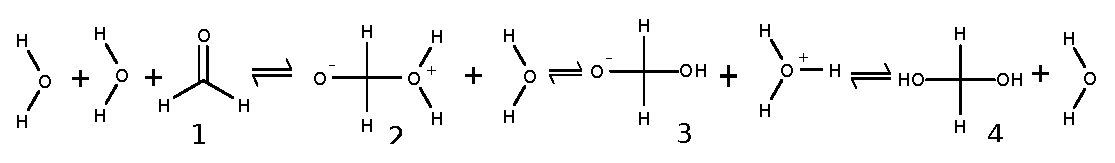
\includegraphics[width=1\textwidth]{formaldehyde2}
  \caption{The most common path through hydration of formaldehyde}
  \label{fig:formal2}
\end{figure}

The carbon in the formaldehyde has a positive partial charge and the oxygen in the water is attracted by 
the carbon and forms a bond to the carbon. This bond is formed out of the electrons of one of the lone 
pairs of the oxygen. 
Since the carbon cannot have more than four bonds this reaction is compensated by 
the double bond in the formaldehyde becoming a single bond and the electrons from the double bond 
forming a lone pair on the oxygen (which now has three lone pairs). These movements are 
concerted, namely they happen together without a stable intermediate state
and cannot be separated. The resulting intermediate (denoted by 2 in Figure~\ref{fig:formal2}) 
has one oxygen which is negatively charged, whereas the other oxygen is positively 
charged. The intermediate 2 abstracts one of the hydrogens to the positively charged oxygen. 
This leads to the intermediate 3 and a $\mathrm{H_3O}$ molecule, 
a water with and additional hydrogen and a positively charged oxygen. One of these hydrogens can be 
re-donated to the negatively charged oxygen. We then get the final products:
methanediol and a molecule of water.

\subsection{The most common path through the reaction}

We shall represent the formaldehyde molecule and the two water molecules as appropriate 
compositions of hydrogen, oxygen and carbon. We use our general prefixing operator, noting that
$O$ has no weak action:
$$\begin{array}{lllllllll}
H & \bydef & (h;p).H' &\qquad O & \bydef & (o,o,n).O' &\qquad C & \bydef & (c,c,c,c;p).C'
\end{array}$$
Carbon has four strong actions $c$, representing the potential for four covalent bonds, and 
a weak action $p$, standing for a positive partial charge. The oxygen is modelled as a flexible 
element with up to 3 bonds. The action $n$ represents the potential for a negative partial charge. 
The hydrogen has one strong bond $h$ and one weak bond $p$.
We employ subscripts to denote individual copies of actions and atoms.
The synchronisation function is defined as follows: $\gamma(c_i,h_j) =  c_ih_j$ for 
$i \in \{1,\ldots, 4\}$ and $j\in\{1,\ldots,6\}$; $\gamma(c_i,n) = c_in$ for $i \in \{1,\ldots, 4\}$;
$\gamma(h_i,n) = h_in$ and $\gamma(h_i,o_j) = h_io_j$ for $i,j \in \{1,\ldots,6\}$; and 
$\gamma(n,p) = np$.

The three molecules of the reaction are placed in parallel:
$\mathrm{CH_2O \paral H_2O \paral H_2O}$.
Each molecule is a parallel composition of its atoms, and we use restriction to force the atoms to
bond together (and in some cases to stay bonded). We also restrict actions $n,p$ so that they
can only happen together. The reaction starts
from the following initial configuration, where keys $1, \ldots, 8$ specify the bonds existing
initially among the atoms of formaldehyde and the two waters. 
%
\begin{flalign*}
&\bigl( (c_1[1],c_2[2],c_3[3],c_4[4];p).C' \paral (h_1[1];p).H'_1 \paral (h_2[2];p).H'_2 \paral 
	(o_1[3],o_2[4],n).O'_1\\ 
& \paral (h_3[5];p).H'_3 \paral (h_4[6];p).H'_4 \paral (o_3[5],o_4[6],n).O'_2 \\
& \paral (h_5[7];p).H'_5 \paral (h_6[8];p).H'_6 \paral (o_5[7],o_6[8],n).O'_3\bigr) 
  \; \setminus L
\end{flalign*}
%
We have grouped all restricted actions at the outer-most level 
and $L$ is $\{c_1,c_2,c_3,\\
c_4,h_1,h_2,h_3,h_4,h_5,h_6,o_1,o_2,o_3,o_4,o_5,o_6,n,p,
\underline{c_{1}h_{1}}, \underline{c_{2}h_{2}}\}$.
%
Apart from the restrictions of the appropriate versions of the $c_i, o_j$ and $h_k$ actions, 
we also restrict $\underline{c_i h_i}$ for $i\in\{1,2\}$. It prevents
breaking any of the bonds between $C_1$ and its hydrogens $H_1,H_2$.
This serves two purposes. Firstly, it makes sure that once we have done the $p$ action of
the carbon, we will break one of the bonds between the carbon and the oxygen. This is justified 
since in reality it is one of the oxygen bonds which is broken. 
Secondly, it also prevents $O_2$ or $O_3$ from abstracting $H_1$ or $H_2$ from the carbon.

We now model the reactions in Figure~\ref{fig:formal2}. The first step is the $n,p$ 
reaction between $C_1$ and $O_2$ or $O_3$. There are other $n,p$ reactions that are allowed
by our model: we describe them in Section~\ref{otherpaths}.
We assume that $O_2$ bonds with $C_1$ with key $9$, followed immediately by breaking of the bond 
3 or 4. Note that breaking of 1 or 2 is not possible because of the restriction on 
breaking $c_1h_1$ and $c_2h_2$. 
Without a loss of generality we break bond 4.
These two partial reactions give us a concerted transition: we create the bond $np[9]$ 
and break the bond $\underline{c_4o_2}[4]$:
%
\begin{flalign*}
&\xrightarrow{\{np[9],\underline{c_4o_2}[4]\}}\bigl((c_1[1],c_2[2],c_3[3],c_4;p[9]).C' \paral 
	(h_1[1];p).H'_1 \paral (h_2[2];p).H'_2 \paral \\
&\qquad (o_1[3],o_2,n).O'_1 
\paral (h_3[5];p).H'_3 \paral (h_4[6];p).H'_4 \paral (o_3[5],o_4[6],n[9]).O'_2 \\
&\paral (h_5[7];p).H'_5 \paral (h_6[8];p).H'_6 \paral (o_5[7],o_6[8],n).O'_3 \bigr) \setminus L
\end{flalign*}
%
Next, we promote the bond 9 of the carbon on a weak $p$ to a stronger bond on $c_4$,
which has become available. Using prom in Definition~\ref{def:reduction} we obtain
%
\begin{flalign*}
&\Rightarrow \; \bigl((c_1[1],c_2[2],c_3[3],c_4[9];p).C' \paral (h_1[1];p).H'_1 \paral 
	(h_2[2];p).H'_2 \paral (o_1[3],o_2,n).O'_1 \\
&\paral (h_3[5];p).H'_3 \paral (h_4[6];p).H'_4 \paral (o_3[5],o_4[6],n[9]).O'_2 \\
&\paral (h_5[7];p).H'_5 \paral (h_6[8];p).H'_6 \paral (o_5[7],o_6[8],n).O'_3 \bigr) \setminus L
\end{flalign*}
%
We note that $O_1$ is now negatively charged (it has only one bond), but we do not need to 
consider it to get our desired result. The next step is to form a bond between $O_3$ and
either $H_3$ or $H_4$. We bond with $H_3$ with key 10 and break the bond 5, producing a pair
of concerted actions. We then promote a weak bond 9 on $n$ in $O_2$ using rule move
from Definition~\ref{def:reduction} to a strong bond
on $o_3$ which has become available. Also, we promote a weak bond 10 in $H_3$ to a
strong bond on $h_3$, and, by the structural congruence rule in Figure~\ref{fig:sc}, we derive 
the transition
%
\begin{flalign*}
&\xrightarrow{\{np[10],\underline{h_3o_3}[5]\}}\bigl((c_1[1],c_2[2],c_3[3],c_4[9];p).C' 
\paral (h_1[1];p).H'_1 \paral (h_2[2];p).H'_2 \paral \\
&\qquad (o_1[3],o_2,n).O'_1 \paral (h_3[10];p).H'_3 \paral (h_4[6];p).H'_4 \paral (o_3[9],o_4[6],n).O'_2 \\
&\paral (h_5[7];p).H'_5 \paral (h_6[8];p).H'_6 \paral (o_5[7],o_6[8],n[10]).O'_3\bigr) \setminus L .
\end{flalign*}
%
The next step is a proton transfer from $O_3$ to $O_1$. We transfer $H_5$, but we could have used 
$H_6$ or $H_3$ since they all have the $p$ action ready. 
Performing the transfer of $H_5$ from $O_3$ to $O_1$ (and breaking the bond 7), we obtain
%
\begin{flalign*}
&\xrightarrow{\{np[11],\underline{h_5o_5}[7]\}}\bigl((c_1[1],c_2[2],c_3[3],c_4[9];p).C' 
	\paral (h_1[1];p).H'_1 \paral (h_2[2];p).H'_2 \paral \\
&\qquad (o_1[3],o_2,n[11]).O'_1 \paral (h_3[10];p).H'_3 \paral (h_4[6];p).H'_4 \paral (o_3[9],o_4[6],n).O'_2 \\
&\paral (h_5;p[11]).H'_5 \paral (h_6[8];p).H'_6 \paral (o_5,o_6[8],n[10]).O'_3 \bigr) \setminus L
\end{flalign*}
and promoting the bond 10 in $O_3$ by the rule move and the bond 11 in $H_5$ by rule prom
we obtain the final products of the reaction:
%
\begin{flalign*}
&\bigl((c_1[1],c_2[2],c_3[3],c_4[9];p).C' \paral (h_1[1];p).H'_1 \paral (h_2[2];p).H'_2 
	\paral (o_1[3],o_2[11],n).O'_1\\
&\paral (h_3[10];p).H'_3 \paral (h_4[6];p).H'_4 \paral (o_3[9],o_4[6],n).O'_2 \\
&\paral (h_5[11];p).H'_5 \paral (h_6[8];p).H'_6 \paral (o_5[10],o_6[8],n).O'_3 \bigr) \setminus L
\end{flalign*}
We have methanediol $\mathrm{CH_2(OH)_2}$ and a molecule of water (oxygen $O_3$ plus hydrogens
$H_6$ and $H_3$).
Note that the $n,p$ actions are ready again and all the existing bonds are on strong actions. 
So we can now reverse the reaction by getting $O_3$ to abstract a hydrogen from $H_4$ or $H_5$. 

Finally, let us inspect the bonds with keys 4, 5 and 7 which are broken during this sequence of
reactions. These bonds were formed prior to the reaction starting. They are broken as a
result of application of our new general prefixing operator. This operator,
in conjunction with the driving forces of the partial charges, guides the reaction without 
relying on any sort of global memory or global control. This is one the main advantages of our
approach.

\subsection{Other paths through the reaction}\label{otherpaths}

There are two other less common ways in which the hydration of formaldehyde in water can happen. 
They require an additional molecule of water.
The three paths through the reaction are shown in Figure~\ref{fig:formal_graph}, now with three waters. 
The path in Figure~\ref{fig:formal2} is from $\mathrm{FA \paral W \paral W \paral W}$ via 
$\mathrm{i2 \paral W \paral W}$ and
$\mathrm{i3 \paral H_3O \paral W}$ where FA stands for formaldehyde, W is water, i2 and i3 are the
intermediates 2 and 3 in Figure~\ref{fig:formal2} and MD is methanediol. 
The other two paths start with an interaction of two water molecules which involves 
a hydrogen transfer and which leads to $\mathrm{FA \paral W \paral HO \paral H_3O}$. The reaction now branches:
either the HO interacts with the formaldehyde, which takes us to $\mathrm{i3 \paral H_3O \paral W}$
and then we follow the remainder of the main path, or we can go via a more complicated sequence of
reactions. The $\mathrm{H_3O}$ interacts with the formaldehyde, then a water molecule attaches 
and finally an interaction with HO brings us to the final state. 
As we can see all the reactions but one are driven 
by concerted actions.

We note that in this example the rates of the individual reactions, and the overall 
rates achieved through the various paths, vary because of the change of energy in the products 
compared to the reactants. We have decided not to model rates at this stage but rather
to concentrate on obtaining all possible valid reactions. We also do not consider
spatial arrangement of molecules.

\begin{figure}[t]
	\psfrag{l1}{${\scriptstyle\{np,\underline{c_4o_2}\}}$}
	\psfrag{l2}{${\scriptstyle\{np,\underline{h_3o_3}\}}$}
	\psfrag{l3}{${\scriptstyle\{np,\underline{h_5o_5}\}}$}
	\psfrag{l4}{${\scriptstyle\{np,\underline{h_3o_3}\}}$}
	\psfrag{l5}{${\scriptstyle\{np,\underline{c_4o_2}\}}$}
	\psfrag{l6}{${\scriptstyle\{np,\underline{h_5o_5}\}}$}
	\psfrag{l7}{${\scriptstyle{np,\underline{c_4o_2}}}$}
	\psfrag{l8}{${\scriptstyle\{np,\underline{h_7o_7}\}}$}
	\psfrag{l9}{${\scriptstyle\{np,\underline{h_8o_8}\}}$}

	\psfrag{fawww}{$\mathrm{FA \paral W \paral W \paral W}$}
	\psfrag{fawhoh3o}{$\mathrm{FA \paral W \paral HO \paral H_3O}$}
	\psfrag{i6whow}{$\mathrm{i6 \paral W \paral HO \paral W}$}
	\psfrag{i8how}{$\mathrm{i8 \paral HO \paral W}$}
	\psfrag{mdhoh3o}{$\mathrm{MD \paral HO \paral H_3O}$}
	\psfrag{i2ww}{$\mathrm{i2 \paral W \paral W}$}
	\psfrag{i3h3ow}{$\mathrm{i3 \paral H_3O \paral W}$}
	\psfrag{mdww}{$\mathrm{MD \paral W \paral W}$}

\centering
\makebox[\textwidth][l]{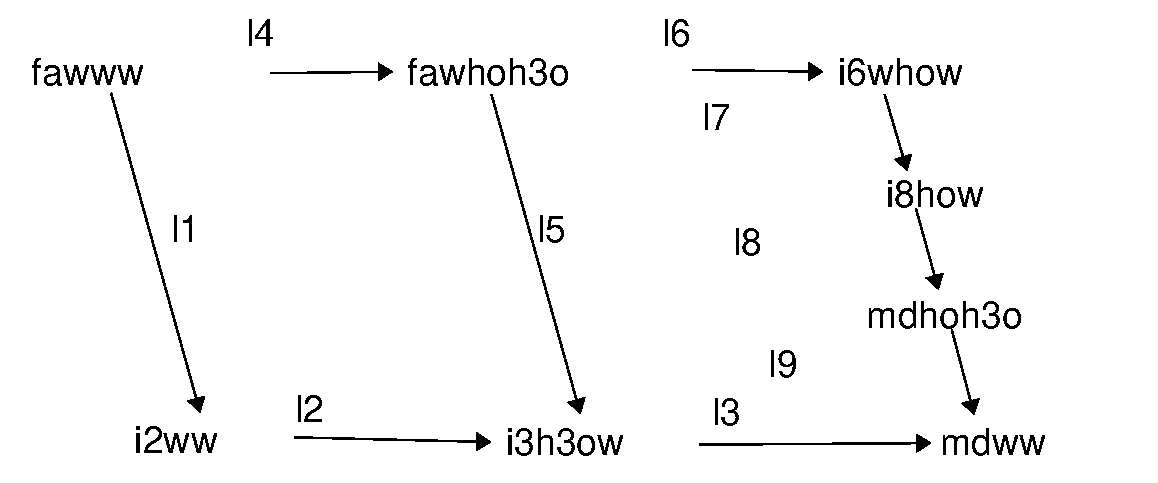
\includegraphics[width=0.9\textwidth]{formal_all}}
\caption{Three paths through hydration of formaldehyde. Communication keys in concerted transitions
are omitted for clarity. The intermediates i6 and i8 are $\mathrm{CH_2O^+H}$ and $\mathrm{COH_3O^+H_2}$
respectively.}
\label{fig:formal_graph}
\end{figure}

\section{Conclusion}
We have introduced a reversible process calculus CCB with a novel prefixing operator which is inspired
by the mechanism of covalent bonding that allows us to model locally controlled reversibility. 
We have given the calculus operational semantics. 
The new operator permits us to perform pairs of concerted actions, where the first element of the pair
is a creation of a (weak) bond and the second element is breaking one of the existing bonds. 
Moreover, our prefixing provides a purely local control of computation; there is no need 
for an extensive memory or global control. We have shown that the sub-calculus 
$\mathrm{CCB_s}$ satisfies conservation and causal consistency, and the full calculus 
satisfies several diamond properties.  CCB is more expressive than other reversible calculi 
as it can also model out-of-causal order computation. We have shown that biochemical reactions 
with covalent bonding can be represented naturally and faithfully thanks to our new prefixing operator
and concerted actions transitions.

\subsubsection*{Acknowledgements}
The authors acknowledge partial support of COST Action IC1405 on Reversible Computation -
extending horizons of computing.

%% The Appendices part is started with the command \appendix;
%% appendix sections are then done as normal sections
%% \appendix

%% \section{}
%% \label{}

%% References
%%
%% Following citation commands can be used in the body text:
%% Usage of \cite is as follows:
%%   \cite{key}          ==>>  [#]
%%   \cite[chap. 2]{key} ==>>  [#, chap. 2]
%%   \citet{key}         ==>>  Author [#]

%% References with bibTeX database:

\bibliographystyle{model1-num-names}
\bibliography{main}

%% Authors are advised to submit their bibtex database files. They are
%% requested to list a bibtex style file in the manuscript if they do
%% not want to use model1-num-names.bst.

%% References without bibTeX database:

% \begin{thebibliography}{00}

%% \bibitem must have the following form:
%%   \bibitem{key}...
%%

% \bibitem{}

% \end{thebibliography}


\end{document}

%%
%% End of file `elsarticle-template-1-num.tex'.
